\section{Digital images and convergent estimators}

\begin{frame}
\huge
\center
Digital images and convergent estimators
\vspace{2em}

\begin{minipage}{0.7\textwidth}
\normalsize
\center
\begin{itemize}
\item{Digital grid particularities and restrictions}
\item{Multigrid convergence of geometric estimators}
\end{itemize}
\end{minipage}

\end{frame}

\begin{frame}
{Digital images and convergent estimators}
{Digital set peculiarities}

\begin{minipage}[t][0.35\textheight][t]{1\textwidth}

Where do we think we can do better?

\only<2->{
\begin{itemize}
\item{Most of models neglect the digital character of digital images and ignore the fact that geometric measurements (mainly those local as tangent and curvature) in such objects should be done with a definition of \emph{convergence} that is specific for digital shapes.}
\end{itemize}
\vspace{1em}

}
\end{minipage}
%
%
\begin{minipage}[t][0.65\textheight][t]{1\textwidth}
\only<3>{
\textbf{Exact sampling x digitization}
\center
\begin{tabular}{ccc}
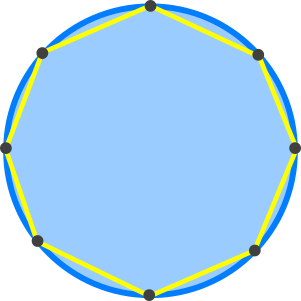
\includegraphics[scale=0.45]{figures/motivation/exact-sampling/sampling-0.png}&
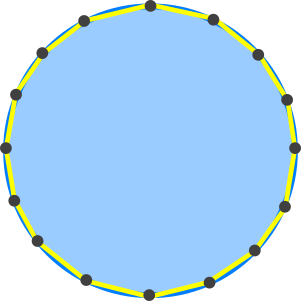
\includegraphics[scale=0.45]{figures/motivation/exact-sampling/sampling-1.png}&
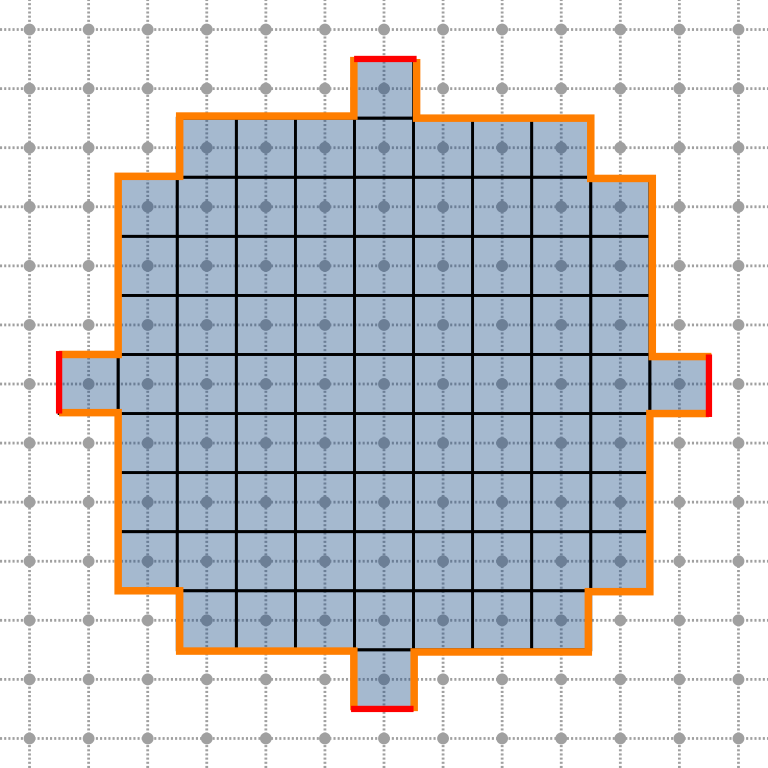
\includegraphics[scale=0.22]{figures/motivation/exact-sampling/digital-ball-perimeter.png}
\end{tabular}}%
\only<4>{
\textbf{Digitization ambiguity}

\begin{center}
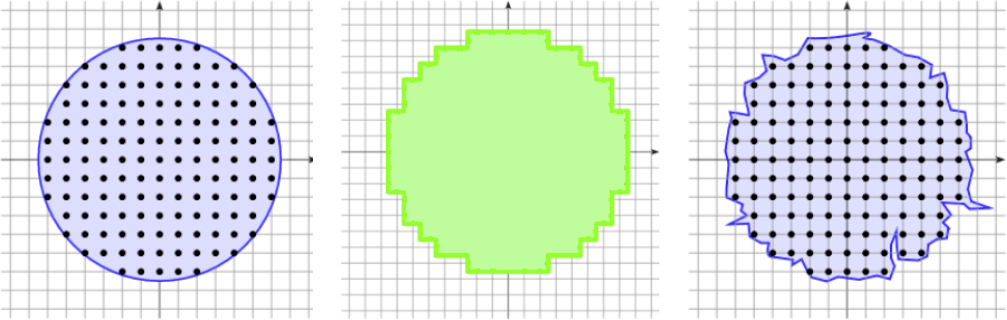
\includegraphics[scale=1]{figures/motivation/exact-sampling/ambiguity.png}
\end{center}}
\end{minipage}
\end{frame}

\begin{frame}
{Digital images and convergent estimators}
{Multigrid convergent estimators}

\begin{definition}[Multigrid convergence]
	Let $\mathcal{X}$ be a family of shapes in $\mathbb{R}^n$ and $u$ a geometric quantity that is defined for every shape $X \in \mathcal{X}$. Further, let $D_h(X)$ denote the digitization of $X$ with grid step $h$.%
%
\vspace{1em}	
%	
	 The estimator $\hat{u}$ is multigrid convergent for $\mathcal{X}$ if and only if, for any $X \in \mathcal{X}$ there exists $h_X > 0$ such that for every $0< h < h_X$
	
	\begin{align*}
		| \hat{u}(D_h(X)) - u(X) | \leq \tau(h), \quad \text{with } \lim_{h\rightarrow 0}{\tau(h)} = 0
	\end{align*}	
\end{definition}
%
\pause
%
Multigrid convergent estimator of area
\begin{align*}
	\widehat{Area(X)} = h^2|D_h(X)|
\end{align*}
%
\end{frame}

\begin{frame}
{Motivation}
{Multigrid convergent estimators}

\footnotesize

\center
Disk of radius $5 (Area\approx78.54)$ 

\center
\begin{tabular}{ccc}
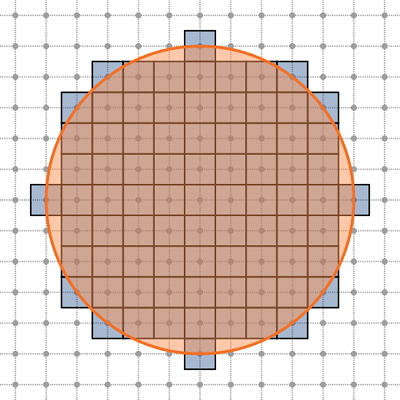
\includegraphics[scale=0.2]{figures/motivation/digital-geometric-estimators/multigrid/h1.png} &
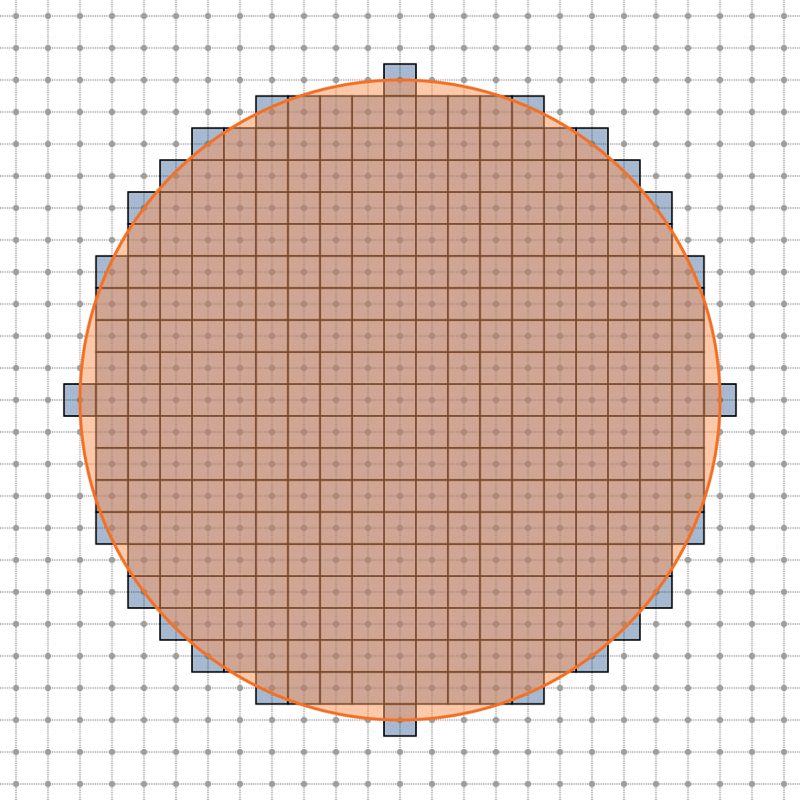
\includegraphics[scale=0.2]{figures/motivation/digital-geometric-estimators/multigrid/h05.png} &
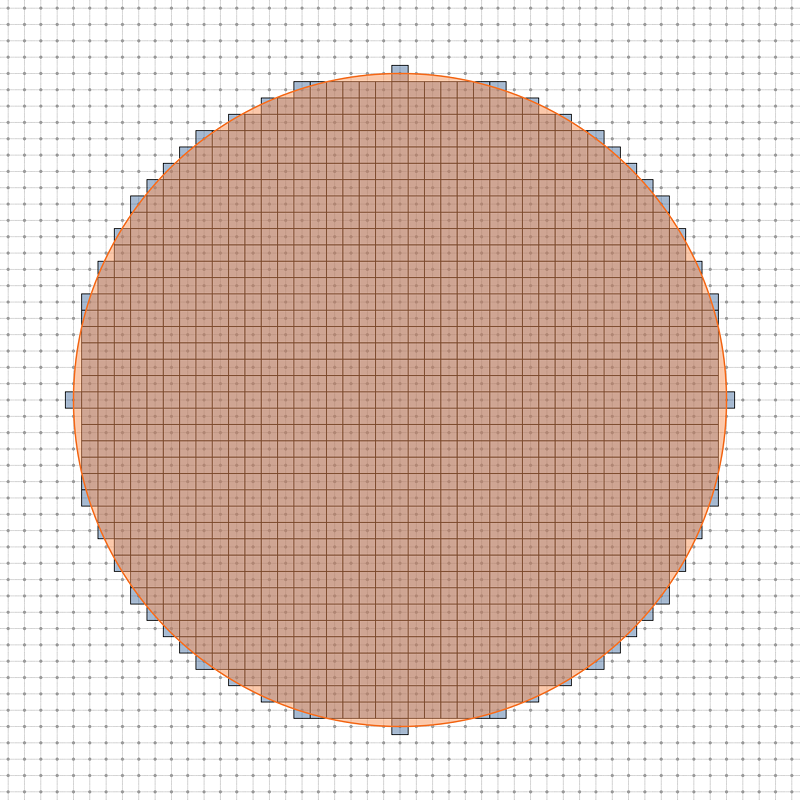
\includegraphics[scale=0.2]{figures/motivation/digital-geometric-estimators/multigrid/h025.png} \\
$h=1.0\; \widehat{A}=81$ & $h=\frac{1}{2}\; \hat{A}=79.25$ & $h=\frac{1}{4}\; \hat{A}=78.56$\\[1em]
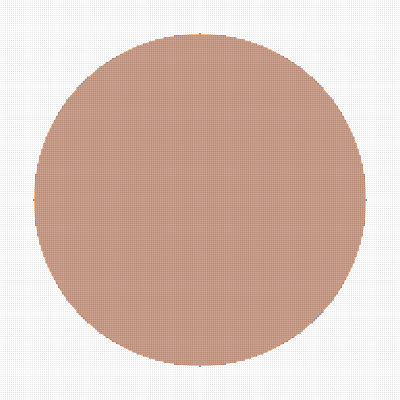
\includegraphics[scale=0.2]{figures/motivation/digital-geometric-estimators/multigrid/h00625.png} &

\includegraphics[scale=0.2]{figures/motivation/digital-geometric-estimators/multigrid/h003125.png} &

\includegraphics[scale=0.2]{figures/motivation/digital-geometric-estimators/multigrid/h003125.png} \\
$h=\frac{1}{16}\; \hat{A}=78.44$ & $h=\frac{1}{32}\; \hat{A}=78.5$ & $h=\frac{1}{64}\; \hat{A}=78.53$
\end{tabular}

\end{frame}

\begin{frame}
	{Digital images and convergent estimators}	
	{Multigrid convergent estimators}	
%
	\begin{itemize}
		\onslide<1->{\item{Minimum Length Polygon (MLP)~\mycite{sloboda98approximation}}
		\begin{itemize}
			\item{Proved multigrid convergent for piecewise $3$-smooth convex shapes.}
		\end{itemize}}
		\onslide<3->{\vspace{2em}
		\item{Integral Invariant (II)~\mycite{coeurjolly13integral}}
		\begin{itemize}
			\item{Proved multigrid convergent for $C^2$ convex shapes with bounded curvature.}
		\end{itemize}}		
	\end{itemize}
	
	\onslide<2>{
	\begin{figure}
	\begin{tikzpicture}[overlay, remember picture] 
	\node at (current page.center) 
	    [
	    anchor=center,
	    xshift=0mm,
	    yshift=0mm
	    ] 
	{
	
	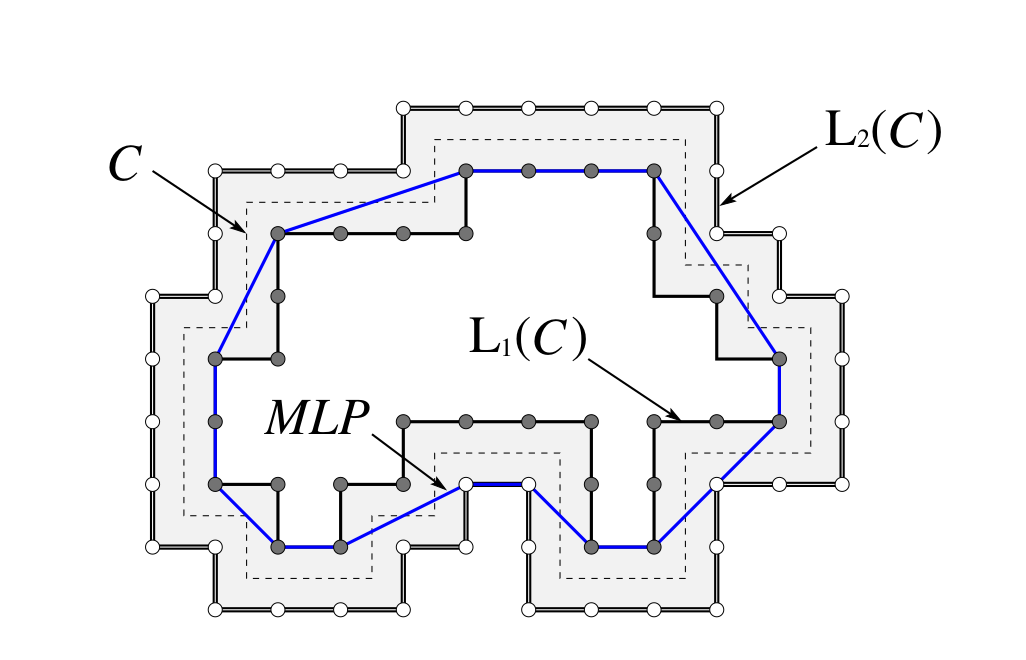
\includegraphics[scale=1.0]{figures/motivation/digital-geometric-estimators/mlp.png}
		
	};
	\end{tikzpicture}	
	\end{figure}	
	}
	
	\onslide<4->{
	\begin{figure}
	\begin{tikzpicture}[overlay, remember picture] 
	\node at (current page.center) 
	    [
	    anchor=center,
	    xshift=0mm,
	    yshift=0mm
	    ] 
	{
	\only<4>{
	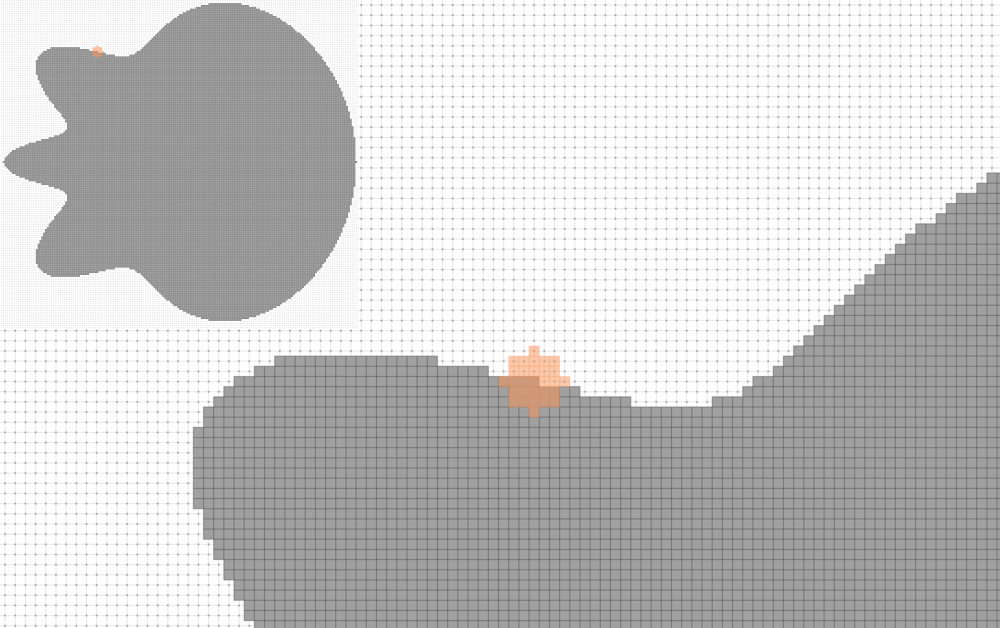
\includegraphics[scale=0.5]{figures/motivation/digital-geometric-estimators/ii/zoom/fr3-zoom.png}}%
	\only<5>{
	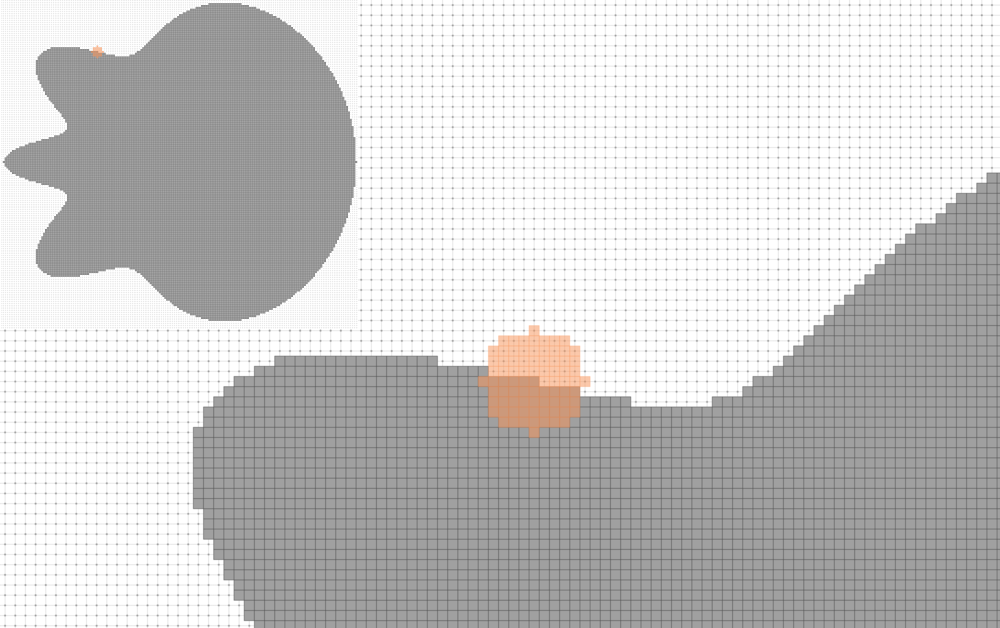
\includegraphics[scale=0.5]{figures/motivation/digital-geometric-estimators/ii/zoom/fr5-zoom.png}}%
		
	};
	\end{tikzpicture}	
	\end{figure}	
	}	

	\vspace{1.5em}

	\onslide<4->{
	\begin{align*}
		\hat{\kappa}(p) = \frac{3}{r^3}\left( \frac{\pi r^2}{2} - | B_r(p) \cap X | \right )
	\end{align*}}		
	
\end{frame}

\begin{frame}
	{Digital images and convergent estimators}	
	{Conclusion}	

	\begin{itemize}
		\item{Digital sets are ambiguous and are constrained to the digital grid.}\\[1em]
		\item{The multigrid convergence is an adapted definition of convergence for geometric estimation on digital sets.}\\[2em]\pause
		\item[]{\textbf{Can we construct optimization models using multigrid convergent estimators?}}
	\end{itemize}

\end{frame}